\subsection{Evaluating the Overhead of Aborted Transactions}
\label{Sec-Eval-Aborted}

The impact of aborted transactions is reported in Tables~\ref{tbl:tsx-stat1} and~\ref{tbl:tsx-stat2}. As the number of threads increases, the number of transactions per successful operation 
also increases, as does the percentage of operations that need more than 10 retries to succeed. 
Note that the innocuous transactions that find inconsistent pointers, changed between the \texttt{SL::find()} and the start of the transaction are not included in the measurement. 
After 10 retries, threads give up on retrying the transactional path and the server executes the operations on their behalf, either in the sequential part, using sequential operations, or in the parallel part, using \texttt{CAS()} for the pointer changes,  but without holding the readers lock. The server does not need to acquire the readers lock because no other thread will try to acquire the writer lock. 


\begin{table}[htb]
\centering
\begin{minipage}{.49\textwidth}
	\centering
  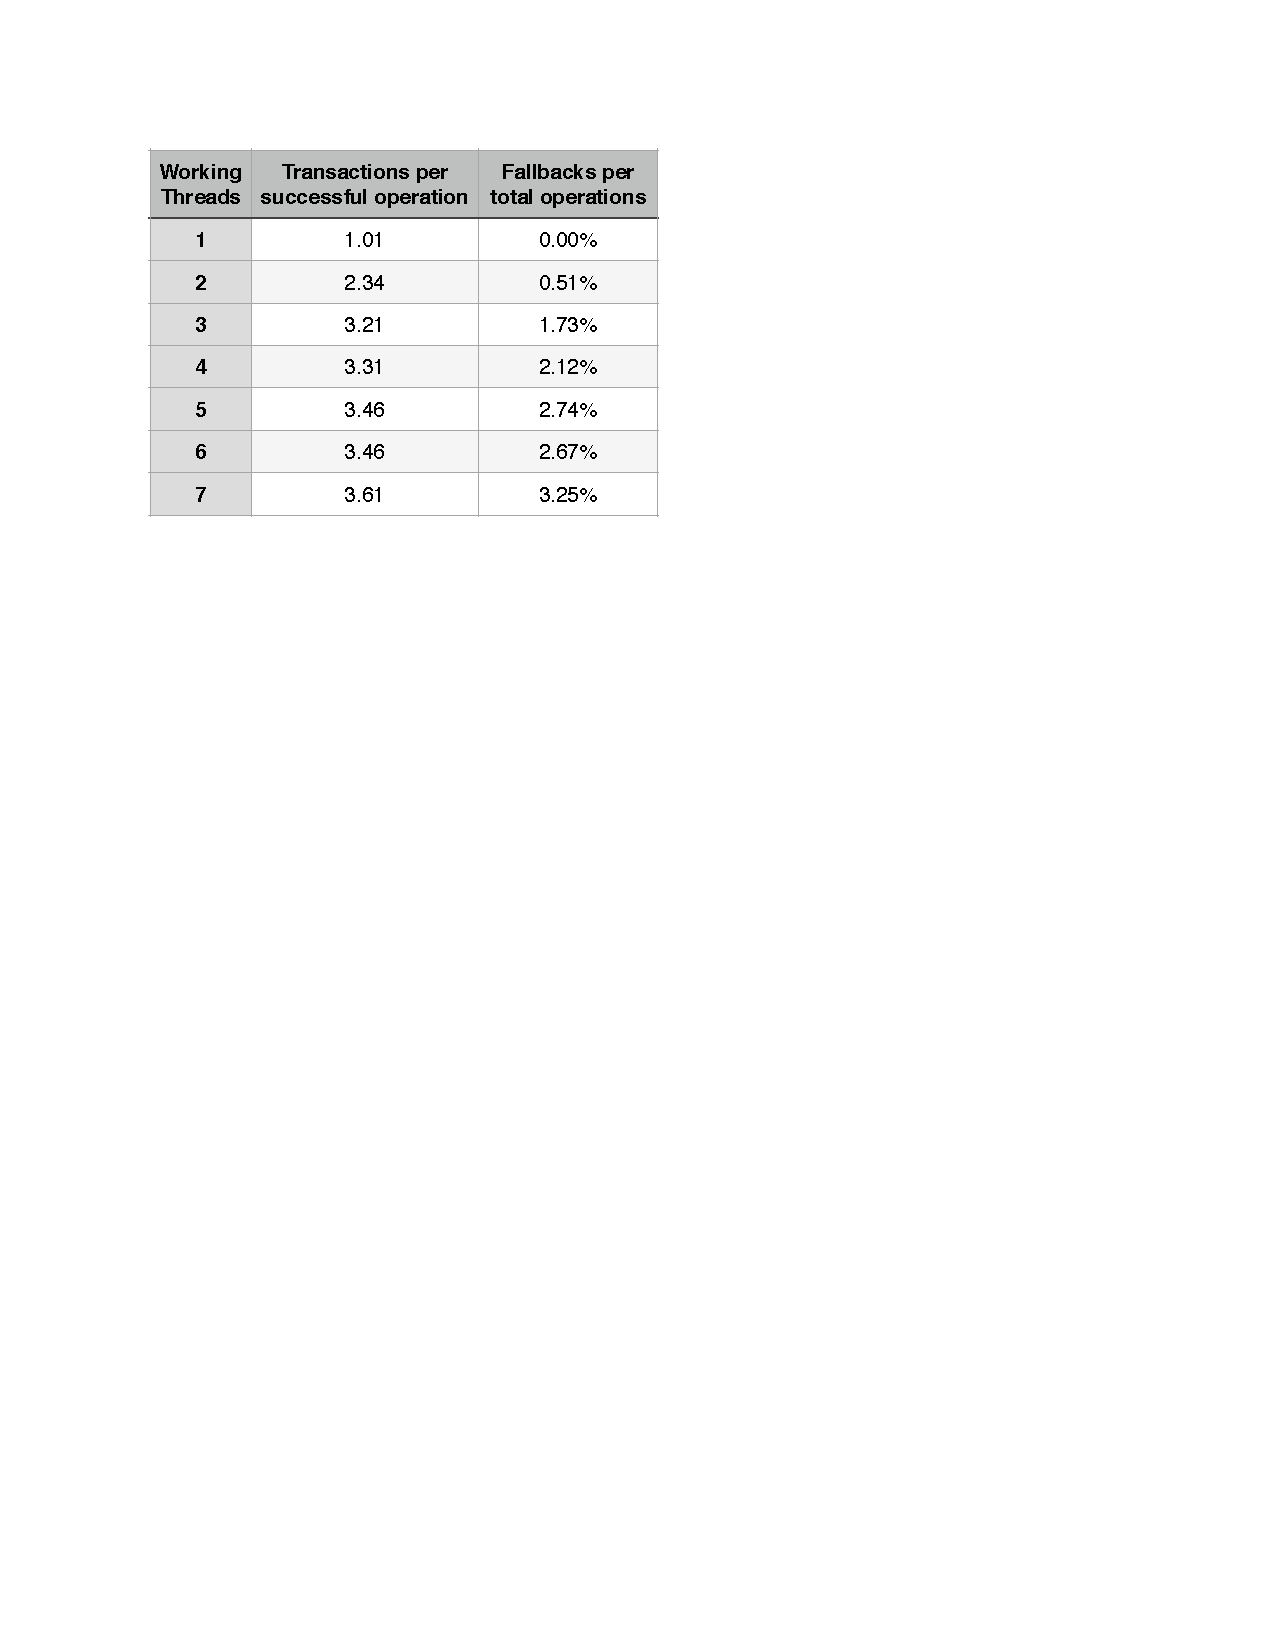
\includegraphics[width=\linewidth]{img/tsx-stat-threads.pdf}
\caption{Transaction stats for varying \# of threads, with 50\% \texttt{PQ::add()}s and 50\% \texttt{PQ::removeMin()}s}
\label{tbl:tsx-stat1}
\end{minipage}%
\hfill%
\begin{minipage}{.49\textwidth}
	\centering
  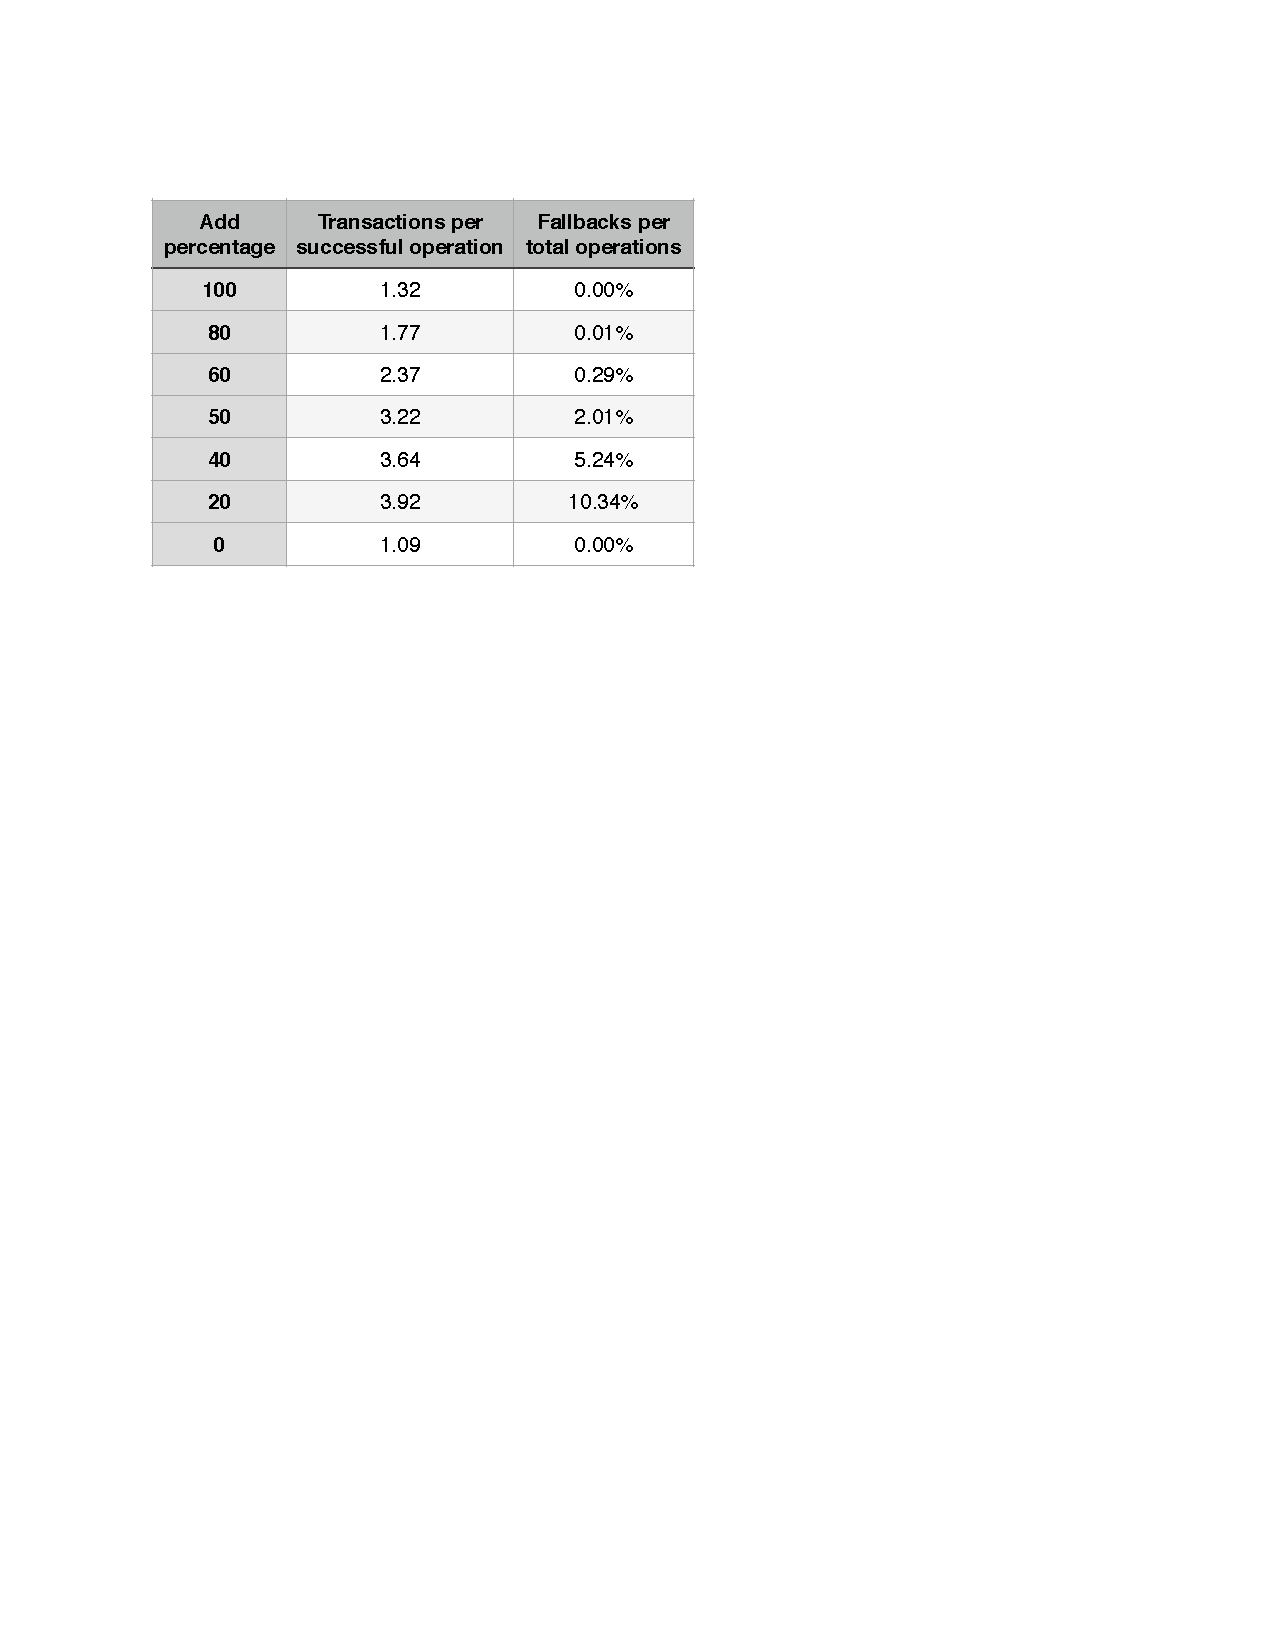
\includegraphics[width=\linewidth]{img/tsx-stat-percents.pdf}
\caption{Transaction stats for varying mixes, with 1 server thread and 3 working threads.}
\label{tbl:tsx-stat2}
\end{minipage}
\caption{Statistics on the overhead of aborted transactions.}
\end{table}

The number of transactions per successful operation is at most $3.92$, but $3.22$ in the $50\%-50\%$ case. The percentage of operations that get executed by the server (after aborting 10 times) is at most $10\%$ of the total number of operations, but between $1.73\%$ and $2.01\%$ for the $50\%-50\%$ case.
